%(BEGIN_QUESTION)
% Copyright 2006, Tony R. Kuphaldt, released under the Creative Commons Attribution License (v 1.0)
% This means you may do almost anything with this work of mine, so long as you give me proper credit

Følgende hydraulikksystem består av tre sylindre koblet sammen med samme rør:

$$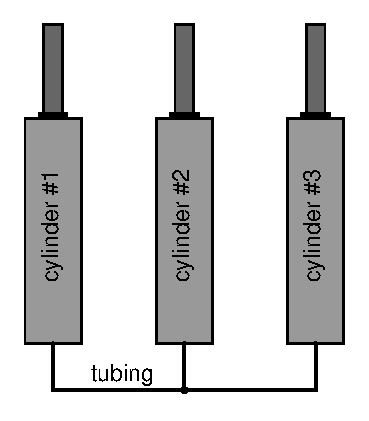
\includegraphics[width=15.5cm]{i00152x01.eps}$$

Forutsatt at alle tre stemplene har samme størrelse: beregn kraften generert av stemplene i sylinder \#2 og \#3 dersom stempelet i sylinder \#1 trykkes med 500 pund kraft.

\underbar{file i00152}
%(END_QUESTION)





%(BEGIN_ANSWER)

Kraften i hvert av de to andre stemplene blir lik: 500 pund. Hvis du tenkte at de 500 pundene på sylinder \#1 skulle deles mellom de to andre stemplene, bør du revurdere trykk/kraft/areal-relasjonen nøye.

%(END_ANSWER)





%(BEGIN_NOTES)

Det som {\it blir} delt mellom de to andre stemplene er {\it forflytning}. Summen av lineær vandring for stempel \#2 og \#3 vil være lik vandringen til stempelet i sylinder \#1.

\vskip 10pt

Hvis studentene dine er komfortable med elektriske kretser, kan denne analogien brukes for å forklare paradokset med lik kraft (500 pund) i hver sylinder:

$$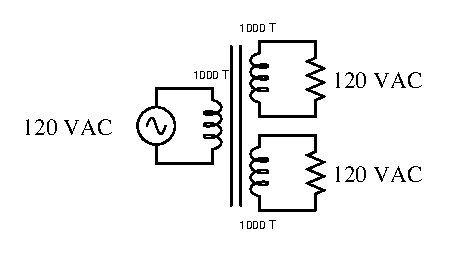
\includegraphics[width=15.5cm]{i00152x02.eps}$$

Tenk på denne skilletransformatoren med tre viklinger og likt antall vindinger (1000 hver). Når den mates med 120 VAC, gir de to sekundærviklingene samme spenning: 120 volt. Spenningen blir {\it ikke} delt mellom sekundærviklingene, akkurat som 500 pund på «master»-stempelet ikke deles mellom «slave»-stemplene.

Derimot blir {\it strøm} delt mellom de to sekundærviklingene, akkurat som {\it forflytning} deles mellom de to slavestemplene. I begge systemer er den bevarte størrelsen {\it energi}. I en tapsfri transformator er effekt ut ($P_{out} = V_{out} I_{out}$) lik effekt inn ($P_{in} = V_{in} I_{in}$). I et tapsfritt master/slave-stempelsystem er arbeid ut ($W_{out} = F_{out} \cdot x_{out}$) lik arbeid inn ($W_{in} = F_{in} \cdot x_{in}$).

%INDEX% Physics, fluids: pressure, force, and area
%INDEX% Physics, static fluids: Pascal's Principle

%(END_NOTES)
